% !TEX program = xelatex
%% Requires compilation with XeLaTeX or LuaLaTeX
\documentclass[10pt,xcolor={table,dvipsnames},t]{beamer}
\usepackage{biblatex}
\usepackage{caption}
\setbeamertemplate{caption}[numbered]
\addbibresource{reference.bib}
\usepackage{hyperref}
\hypersetup{ 
pdfpagemode=FullScreen,  
colorlinks=true,linkcolor=blue}
\usepackage{enumerate}
\usepackage{algorithm}
\usepackage{mathtools}
\usepackage{algpseudocode}
\usepackage{listings}
\usepackage{xcolor}

\definecolor{codegreen}{rgb}{0,0.6,0}
\definecolor{codegray}{rgb}{0.5,0.5,0.5}
\definecolor{codepurple}{rgb}{0.58,0,0.82}
\definecolor{backcolour}{rgb}{0.95,0.95,0.92}

\lstdefinestyle{mystyle}{
    backgroundcolor=\color{backcolour},   
    commentstyle=\color{codegreen},
    keywordstyle=\color{magenta},
    numberstyle=\tiny\color{codegray},
    stringstyle=\color{codepurple},
    basicstyle=\ttfamily\footnotesize,
    breakatwhitespace=false,         
    breaklines=true,                 
    captionpos=b,                    
    keepspaces=true,                 
    numbers=left,                    
    numbersep=5pt,                  
    showspaces=false,                
    showstringspaces=false,
    showtabs=false,                  
    tabsize=2
}

\lstset{style=mystyle}

% Flow chart config
\usepackage{tikz}
\usetikzlibrary{calc,trees,positioning,arrows,fit,shapes,calc,tikzmark,matrix}
\usepackage{eso-pic}
\usetikzlibrary{shapes.geometric, arrows}
\tikzstyle{startstop} = [rectangle, rounded corners, minimum width=3cm, minimum height=1cm,text centered, draw=black, fill=red!30]
\tikzstyle{io} = [trapezium, trapezium left angle=70, trapezium right angle=110, minimum width=3cm, minimum height=1cm, text centered, draw=black, fill=blue!30]
\tikzstyle{process} = [rectangle, minimum width=3cm, minimum height=1cm, text centered, draw=black, fill=orange!30]
\tikzstyle{decision} = [diamond, minimum width=3cm, minimum height=1cm, text centered, draw=black, fill=green!30]
\tikzstyle{arrow} = [thick,->,>=stealth]

\usetheme{UCBerkeley}

\title[Your Short Title]{STMC coding team Training}
\subtitle{Lesson 5: Function and Recursion}
\author{Tsai Yun Chen}
%\institute{}
\date{April 5, 2024}

\begin{document}

\begin{frame}
  \titlepage
\end{frame}

% Uncomment these lines for an automatically generated outline.
%\begin{frame}{Outline}
%  \tableofcontents
%\end{frame}

\section{Class Goal}

\begin{frame}{Goal today}
  Function provides us a way to write code in a clean and organized way, and it provides us ways to solve problems with few lines of code
\begin{itemize}
  \item Introduce function to modularize code
  \item Using function to make previous code cleaner
  \item Function as parameter, Function Folding
  \item Introduce recursion: Divide and Conquer
  \item Merge Sort
  \item Fibonacci number
  \item Problem of Recursion
  \item Strategy of Memoization
  \item Fibonacci number, revised
\end{itemize}

\end{frame}

\section{Function}
\begin{frame}[fragile]{Code Reusability}
  \begin{itemize}
    \item \textbf{Code reuse} is the use of existing software, or software knowledge, to build new software 
    \item Many times in programming, certain segment of code (e.g. search for name in contact for example) will be used again and again 
    \item We would therefore want to reuse those code without keep typing it again and again 
    \item Here is an example:
  \end{itemize}
\end{frame}

\begin{frame}[fragile]
\begin{lstlisting}[language=python]
# Searching for names in contact

contact = ['Billy','Damon','Leon','Mary','Shirley']
searchName = input('Enter a name: ')
inContact = False 
for name in contact:
  if searchName == name:
    inContact = True 
if inContact:
  print(f'{searchName} is in contact')

# Search another one
searchName = input('Enter a name again: ')
inContact = False 
for name in contact:
  if searchName == name:
    inContact = True 
if inContact:
  print(f'{searchName} is in contact')
  \end{lstlisting}
\end{frame}

\begin{frame}[fragile]{Code Reusability}
  \begin{itemize}
    \item As shown in the code, line 13 to 19 is completely identical to the above
    \item It would be great if we can put them into one line like this:
\begin{lstlisting}[language=python]
if haveName(contact, name):
  print(f'{name} is in contact')
\end{lstlisting}
    \item \textit{function} provide exactly what we want
  \end{itemize}
\end{frame}

\begin{frame}{Function}
  \begin{columns}
    \begin{column}[T]{0.6\textwidth}
      \begin{itemize}
        \item \textbf{Function}, in the simplest term, is a machine that takes in some input $x$ and perform some action on $x$, producing an output $f(x)$
        \item For example, we may define the following functions:
        \begin{itemize}
          \item $f(x) = x^2$
          \item $f(x) = x^x$
          \item $f(x) = \text{Last digit of x in decimal}$
          \item $f(x) = \{x \quad \text{if} \quad x\geq 0, -x \quad \text{if} \quad x < 0\}$
          \item $f(x,y) = xy^2 + x^2 y^4$
        \end{itemize}
      \end{itemize}
    \end{column}
    \begin{column}[T]{0.4\textwidth}
      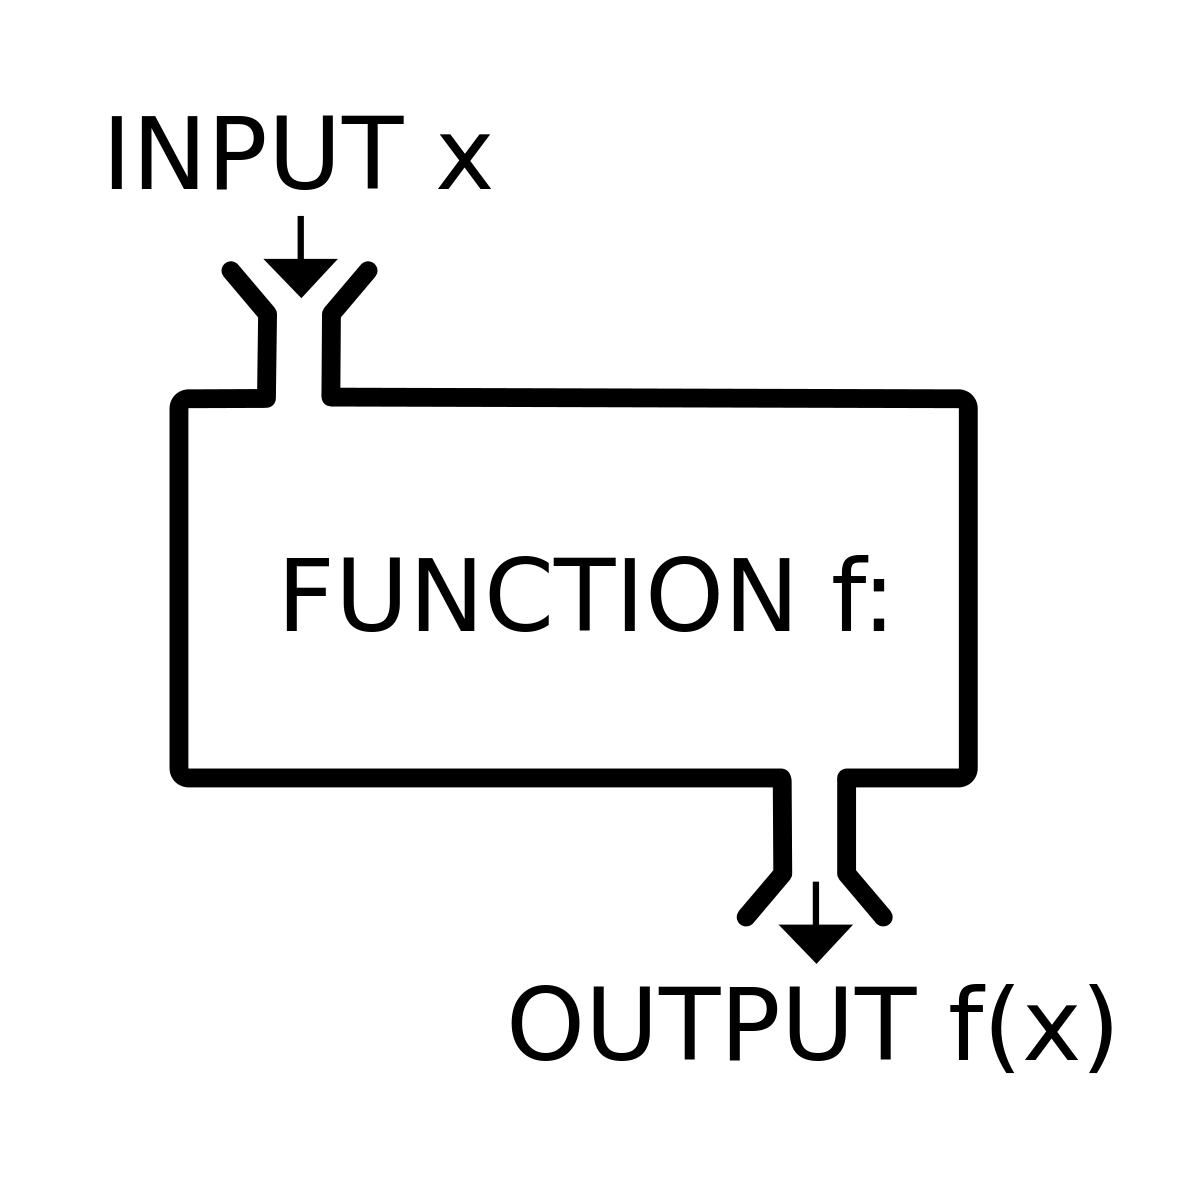
\includegraphics[width=\textwidth]{img/function_as_machine.png}
    \end{column}
  \end{columns}
\end{frame}

\begin{frame}{Function}
  \begin{itemize}
    \item To \textit{evaluate} a function, we put in an input and perform the actions as described by the definition of the $f$. For example:
    \begin{table}[]
      \begin{tabular}{cccc}
                               & \multicolumn{3}{c}{$f(x)$}                                                                            \\ \cline{2-4} 
      \multicolumn{1}{c|}{$x$} & \multicolumn{1}{c|}{$x^2$}    & \multicolumn{1}{c|}{$x^x$}         & $x$ if $x\geq 0$, $-x$ otherwise \\ \hline
      \multicolumn{1}{c|}{-1}  & \multicolumn{1}{c|}{$(-1)^2$} & \multicolumn{1}{c|}{$(-1)^{(-1)}$} & 1                                \\ \cline{1-1}
      \multicolumn{1}{c|}{1}   & \multicolumn{1}{c|}{$(1)^2$}  & \multicolumn{1}{c|}{$(1)^{(1)}$}   & 1                                \\ \cline{1-1}
      \multicolumn{1}{c|}{2}   & \multicolumn{1}{c|}{$(2)^2$}  & \multicolumn{1}{c|}{$(2)^{(2)}$}   & 2                                \\ \cline{1-1}
      \multicolumn{1}{c|}{11}  & \multicolumn{1}{c|}{$(11)^2$} & \multicolumn{1}{c|}{$(11)^{(11)}$} & 11                              
      \end{tabular}
      \end{table}
  \end{itemize}
\end{frame}

\begin{frame}{Function}
  \begin{itemize}
    \item By defining functions, we can simply expressions by "calling" them in our expressions 
    \item For example, 
    $$\text{max}(a,b) = \frac{|a-b|+(a+b)}{2}$$
    gives the larger number between $a$ and $b$. (Why?)
    \item By nesting $\text{max}$ we can perfrom find max between more number
    $$f(a,b,c,d) = \text{max}(\text{max}(a,b),\text{max}(c,d))$$
  \end{itemize}
\end{frame}

\begin{frame}{Functions in programming}
  \begin{itemize}
    \item In programming, functions are "self contained" modules of code that accomplish a specific task.
    \item A function takes in certain inputs called the \textbf{arguments} and produce outputs called \textbf{return value}
    \item For example, you may write a \texttt{UserLookup} function that takes in the username as argument, and return user info as return value.
  \end{itemize}
\end{frame}

\begin{frame}[fragile]{Function in programming}
  \begin{itemize}
    \item In python, a function have the following syntax
\begin{lstlisting}[language=python]
def func(arg1,arg2,...):
  # Operations
  return val1,val2,...
\end{lstlisting}
  \item For example, the \texttt{max} function just now:
\begin{lstlisting}[language=python]
def max(a,b):
  return (abs(a-b)+(a+b))/2   #you can also use if-then-else
\end{lstlisting}
  \end{itemize}
\end{frame}

\begin{frame}{Function Exercises}
  Complete the following exercises
  \begin{enumerate}
    \item Write a function \texttt{Square(x)} that square a number 
    \item Write a function \texttt{SumAll(num\_list)} that return the sum of a list of numbers \texttt{num\_list}
    \item Write a function \texttt{MinMax(num\_list)} that returns the mininum number from the list \texttt{num\_list}
    \item Write a function \texttt{Reverse(str)} that returns the reverse of the string
  \end{enumerate}
\end{frame}

\begin{frame}{Folding}
  \begin{itemize}
    \item Observe in the last few tasks, we are repeating something similar as well!
    \item We walk through the list and do something to each elements
    \item Can we make this as a function as well?
    \item Yes! This trick is called function folding
  \end{itemize}
\end{frame}

\begin{frame}[fragile]{Function Left Folding}
\begin{lstlisting}[language=python]
def LeftFold(list,func):
  first=False
  for item in list:
    if first:
      res=item
      first=True
    else:
      res=func(res,item)
  return res
\end{lstlisting}
\end{frame}

\begin{frame}[fragile]{Example of using folding}
\begin{lstlisting}[language=python]
  def max(a,b):
    return (abs(a-b)+(a+b))/2
  
  def sum(a,b):
    return a+b
  
  list=[3,7,11,99,34,5,16]

  print("The maximum of elements of the list:",LeftFold(list,max))
  print("The sum of elements of the list:",LeftFold(list,sum))
\end{lstlisting}
\end{frame}

\section{Recursion}

\begin{frame}[fragile]{Recursion: Divide and Conquer}
  \begin{itemize}
    \item Some times problems can be divided into several parts
    \item Each parts are actually the same problem, but smaller
    \item example sorting, permutation, counting etc.
    \item Recursion is a kind of trick that solve the problem by first solving its smaller sub-problem
  \end{itemize}
\end{frame}

\begin{frame}[fragile]{Recursion}
  \begin{columns}
    \begin{column}{0.6\textwidth}
      \begin{itemize}
        \item Function also allow us to easily implement algorithms that involve \textbf{recursion}
        \item That is, solutions that depends on solutions to smaller instances of the same problem
        \item As we will illustrate, recursion sometimes allow us to solve complicated problems in very neat way
      \end{itemize}
    \end{column}
    \begin{column}[T]{0.4\textwidth}
      \begin{figure}
        
        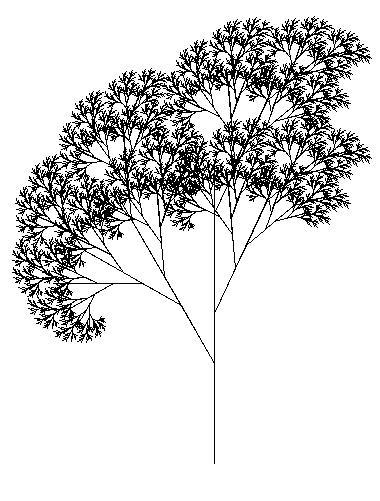
\includegraphics[width=0.7\textwidth]{img/RecursiveTree.JPG}
        \caption{Recursive Tree (\href{https://upload.wikimedia.org/wikipedia/commons/f/f7/RecursiveTree.JPG}{Source})}
      \end{figure}
    \end{column}
  \end{columns}
\end{frame}

\begin{frame}{Example: Merge Sort}
  \begin{itemize}
    \item Recall we discussed about how we can sort a list using looping
    \item We also discussed about the time needed for the naive soring: $O(n^{2})$.
    \item Now we discuss a recursive approach
  \end{itemize}
\end{frame}

\begin{frame}{Example: Merge Sort}
  \begin{itemize}
    \item The first step is to find the sub-problem
    \item Let's say we separate our array into two halves
    \item Then we sort them separately
    \item Can we merge the two sorted arrays?
  \end{itemize}
\end{frame}

\begin{frame}{Example: Merge Sort}
  \begin{itemize}
    \item Let's try, consider having an array $$\{11,6,4,2,7,18,1,21\}$$
    \item Now separate it into two halves, $$\{11,6,4,2\},\{7,18,1,21\}$$
    \item sort them separately, $$\{2,4,6,11\},\{1,7,18,21\}$$
    \item How do we merge them? Take the smaller of them! (Greedy)
  \end{itemize}
\end{frame}

\begin{frame}{Example: Merge Sort}
  \begin{columns}
    \begin{column}{0.6\textwidth}
      \begin{itemize}
        \item But wait! How do we sort the two smaller array?
        \item Look back to our original problem, what are we solving? Sorting!
        \item Let's run the same function on the smaller array again.
        \item But when do we stop?
        \item If an array contains only one element, then it must be sorted.
      \end{itemize}
    \end{column}
    \begin{column}[T]{0.4\textwidth}
      \begin{figure}
        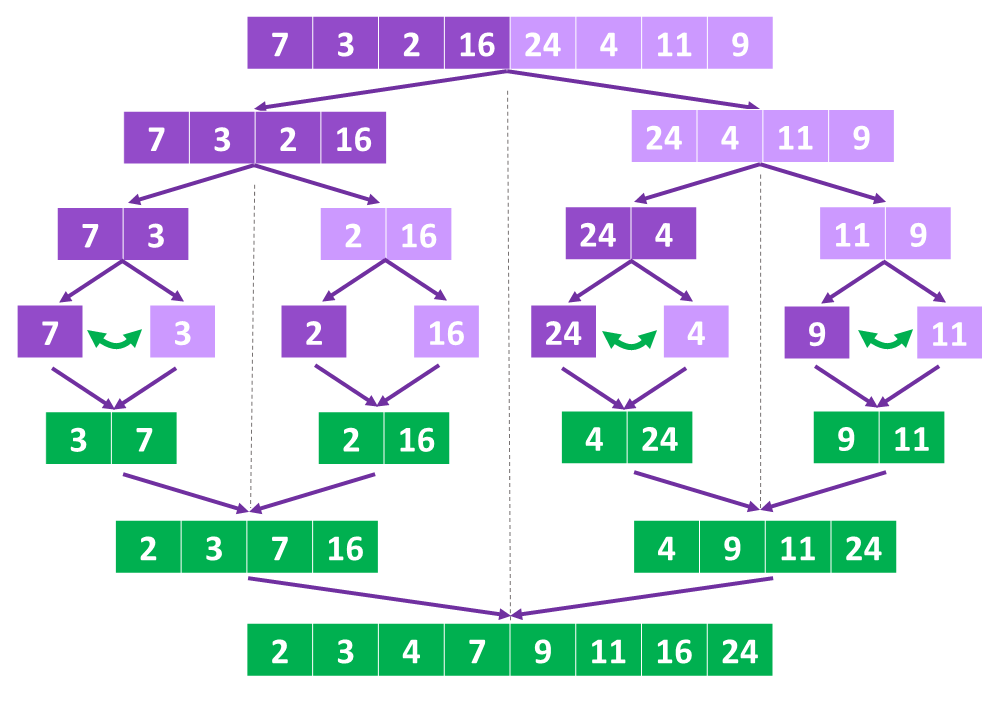
\includegraphics[width=0.7\textwidth]{img/Merge-Sort.png}
        \caption{Merge Sort (\href{https://www.101computing.net/merge-sort-algorithm/}{Source})}
      \end{figure}
    \end{column}
  \end{columns}
\end{frame}

\begin{frame}[fragile]
\begin{lstlisting}[language=python]
def MergeSort(list):
  length=len(list)
  if length==1:
    return list
  left=list[0:length//2]
  right=list[(length//2):length]
  LeftSorted=MergeSort(left)
  RightSorted=MergeSort(right)
  listSorted=[]
  LPointer=0
  RPointer=0
  for i in range(length):
    if RPointer==len(RightSorted):
      listSorted.append(LeftSorted[LPointer])
      LPointer=LPointer+1
    elif LPointer==len(LeftSorted) or RightSorted[RPointer]<LeftSorted[LPointer]:
      listSorted.append(RightSorted[RPointer])
      RPointer=RPointer+1
    else:
      listSorted.append(LeftSorted[LPointer])
      LPointer=LPointer+1
  return listSorted
\end{lstlisting}
\end{frame}

\begin{frame}{Example: Fibonacci Sequence}
  \begin{itemize}
    \item Recall the Fibonacci sequence that we discuss long time ago
    \begin{align*}
        &F(n+2) = F(n+1) + F(n)\\
        &F(1) = F(2) = 1
    \end{align*}
    \item We had implemented that using loops before, we will now try to do it in recursion 
  \end{itemize}
\end{frame}

\begin{frame}[fragile]{Example: Fibonacci Sequence}
  \begin{lstlisting}[language=python]
# Fibonacci sequence using recursion
def Fib(n):
  if n == 1 or n == 2:
    return 1
  else:
    return Fib(n-1) + Fib(n-2)
  \end{lstlisting}
\end{frame}


\begin{frame}{Example: Fibonacci Sequence}
  \begin{itemize}
    \item As shown in the code, calling $F(4)$ returns $F(3)+F(2)$ 
    \item To return $F(3)+F(2)$, we must evaluate $F(3)$ and $F(2)$
    \item $F(2)$ by line 3,4 of the code returns $1$
    \item $F(3)$ on the otherhand calls $F(1)+F(2)$, which both evaluates to $1$ according to line 3,4
    \item So we "backsubstitute" the values layer by layer up and evaluate $F(4) = ((1+1)) + (1) = 3$
  \end{itemize}
\end{frame}

\begin{frame}{Example: Fibonacci Sequence}
  \begin{itemize}
    \item To see what happens for larger $n$, we can consider the following figure
    \begin{figure}
      \centering
      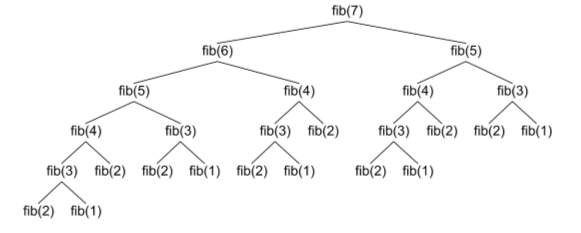
\includegraphics[width=0.8\textwidth]{img/fib-tree.png}      
      \caption*{Source: \href{https://stackoverflow.com/questions/35959100/explanation-on-fibonacci-recursion}{StackOverflow}}
    \end{figure}
  \end{itemize}
\end{frame}

\begin{frame}{Something is wrong...}
  \begin{itemize}
  \item Look at the tree diagram on previous page, what can you observed?
  \item How many time does fib(5) appear? What about fib(4) and fib(3)?
  \item A problem of recursion is it might solve the same problem repeatly
  \item You might ask, why care about it?
  \end{itemize}
\end{frame}

\begin{frame}{Time complexity of naive Fibonacci recursion}
  \begin{itemize}
    \item Let's see if that really matters.
    \item We let $T(n)$ be the time needed for solving the $n$-th fibonacci number
    \item By the formula, we know that $$T(n)=\underbrace{T(n-1)+T(n-2)}_{\text{computing previous terms}}+\underbrace{\vphantom{T(n-1)+T(n-2)}1}_{\mathclap{\text{addition}}}$$
    \item Solving it (with some tedious math), we get $$T(n)\approx 2^{n}$$
  \end{itemize}
\end{frame}

\begin{frame}{Strategy of Memoization}
  \begin{itemize}
    \item Exponential is almost the worst thing we can get.
    \item Turns out it matters, but how can we improve it?
    \item Simple method: remembering previous result
    \item This approach is called Memoization
  \end{itemize}
\end{frame}

\begin{frame}[fragile]{Fibonacci number, revised}
\begin{lstlisting}[language=python]
# Fibonacci sequence using recursion, with Memoization
def _Fib(n):
  if n == 1 or n == 2:
    return (1,1)
  else:
    prev=_Fib(n-1)
    return (prev[1],prev[0]+prev[1])

def Fib(n):
  pair=_Fib(n)
  return pair[1]
\end{lstlisting}
\end{frame}


  
\begin{frame}{Example: Tower of Hanoi}
  \begin{itemize}
    \item The Tower of Hanoi is a mathematical puzzle first introduced by Édouard Lucas in 1883
    \item It begins with the disks stacked on one rod in order of decreasing size, the smallest at the top, thus approximating a conical shape. 
     \item The objective of the puzzle is to move the entire stack to the last rod, obeying the following rules: 
    \begin{enumerate}
      \item Only one disk may be moved at a time.
      \item Each move consists of taking the upper disk from one of the stacks and placing it on top of another stack or on an empty rod.
      \item No disk may be placed on top of a disk that is smaller than it.
    \end{enumerate}
  \end{itemize}
\end{frame}

\begin{frame}{Exercise: Tower of Hanoi}
\begin{figure}
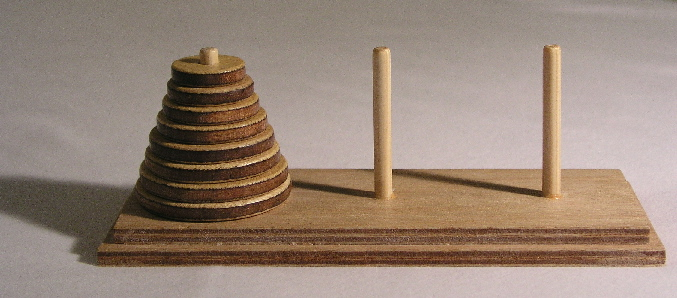
\includegraphics[width=0.8\textwidth]{img/hanoi.jpeg}
\end{figure}
\end{frame}

\begin{frame}{Exercise: Tower of Hanoi}
\begin{itemize}
\item We would like to program an algorithm that would \textit{solves} the tower of hanoi
\item Given a stack of $n$ disk to begin with, derive a program that will teach you how should you move the disks to solve the puzzle
\item Let's try to play around with the game to gain some insights and familiarity
\item Here is a link to the game: \href{https://www.mathsisfun.com/games/towerofhanoi.html}{https://www.mathsisfun.com/games/towerofhanoi.html}
\end{itemize}
\end{frame}

\begin{frame}{Solution: Tower of Hanoi}
\begin{exampleblock}{Observations:}
Suppose there are $n$ disks and suppose we know how to move $n-1$ disks from rod 1 to rod 2. Then to move $n$ disks, we just need to:
\begin{enumerate}
  \item Move all $n-1$ disk above to the rod in the middle rod
  \item Place the bottom disk to the final rod
  \item Move the $n-1$ disks to the final rod 
\end{enumerate}
\end{exampleblock}
\end{frame}

\begin{frame}{Solution: Tower of Hanoi}
\begin{itemize}
\item In other words, once we know how to move $n-1$ disks, moving $n$ disks is easy
\item But how do we know how to move $n-1$ disks?
\item Well, to move $n-1$ disk, we just need to know how to move $n-2$ disks!
\item Wait how about $n-2$? We don't know how to do that right?
\item Well, we just have to figure out how to move $n-3$ disks!
\item $\cdots$
\item But how to move $2$ disks?
\item Well, to move $2$ disks, we just need to know how to move $1$ disk
\item \textbf{But moving 1 disk is trivial!}
\end{itemize}
\end{frame}

\begin{frame}[fragile]{Homework}
  \begin{itemize}
    \item Homework 3 is posted on the course website, namely the HW3.ipynb
    \item same as last time, 3 problems, sorted in ascending order of difficulty
    \item cover topics of looping, list and functions
    \item submit the homework to \href{https://drive.google.com/drive/folders/1TqSFSwu8-KdzIHZcQWB7PjgqPJen4dsO?usp=sharing}{the same place}, inside the folder of \texttt{HW3 submission}
    \item remember to include all your group member's name in the document
    \item deadline: before next lesson, i.e. 13/4
    \item the solution will be disclosed one week after the deadline, i.e. 20/4
    \item comments and solution on HW2 are released.
  \end{itemize}
\end{frame}

\end{document}
